\let\negmedspace\undefined
\let\negthickspace\undefined
\documentclass[journal]{IEEEtran}
\usepackage[a5paper, margin=10mm, onecolumn]{geometry}
%\usepackage{lmodern} % Uncomment if needed for pdflatex
\usepackage{tfrupee} % Include tfrupee package

\setlength{\headheight}{1cm} % Set the height of the header box
\setlength{\headsep}{0mm}     % Set the distance between the header box and the top of the text

\usepackage{gvv-book}
\usepackage{gvv}
\usepackage{cite}
\usepackage{amsmath,amssymb,amsfonts,amsthm}
\usepackage{algorithmic}
\usepackage{graphicx}
\usepackage{textcomp}
\usepackage{xcolor}
\usepackage{txfonts}
\usepackage{listings}
\usepackage{enumitem}
\usepackage{mathtools}
\usepackage{gensymb}
\usepackage{comment}
\usepackage[breaklinks=true]{hyperref}
\usepackage{tkz-euclide} 
\usepackage{listings}
%\usepackage{gvv}                                        
\def\inputGnumericTable{}                                 
\usepackage[latin1]{inputenc}                                
\usepackage{color}                                            
\usepackage{array}                                            
\usepackage{longtable}                                       
\usepackage{calc}                                             
\usepackage{multirow}                                         
\usepackage{hhline}                                           
\usepackage{ifthen}                                           
\usepackage{lscape}
\usepackage{tikz}
\usepackage{circuitikz}
\usepackage{standalone} % For including external TikZ files

\begin{document}

\bibliographystyle{IEEEtran}
\vspace{3cm}

\title{11.16.3.5.2}
\author{EE24BTECH11066 - YERRA AKHILESH}
% \maketitle
% \newpage
% \bigskip
{\let\newpage\relax\maketitle}

\renewcommand{\thefigure}{\theenumi}
\renewcommand{\thetable}{\theenumi}
\setlength{\intextsep}{10pt} % Space between text and floats

\numberwithin{equation}{enumi}
\numberwithin{figure}{enumi}
\renewcommand{\thetable}{\theenumi}

\textbf{Question}:\\ 

A fair coin with 1 marked on one face and 6 on the other and a fair die are both tossed. Find the probability that the sum of numbers that turn up is 12.\\

\textbf{Solution: }\\
\textbf{Textual solution: }\\
The probability of a given event $A$ (where $A$: Sum of the numbers is 12) is computed by considering the mutual independence of the coin and the die. Since the coin and die are independent events, we calculate the probability of each event separately and then multiply them.

The probability of the coin showing 6 is:
\[
P(\text{Coin} = 6) = \frac{1}{2}
\]
The probability of the die showing 6 is:
\[
P(\text{Die} = 6) = \frac{1}{6}
\]

Since the events are independent, the probability of both events happening together is:
\[
P(A) = P(\text{Coin} = 6) \times P(\text{Die} = 6) = \frac{1}{2} \times \frac{1}{6} = \frac{1}{12}.
\]


\textbf{Computational solution: }
\section*{Computation of Probabilities for Tossing a Coin and Rolling a Die}

To compute the probability of obtaining specific outcomes when tossing a fair coin and rolling a six-sided die, we rely on two key concepts: the **Probability Mass Function (PMF)** and the **Cumulative Distribution Function (CDF)**.

\subsection*{Definitions}
\subsubsection*{Probability Mass Function (PMF)}
The PMF represents the probability of each individual outcome in the sample space $S$. For the coin:
\[
C = \{1, 6\}
\]
and for the die:
\[
D = \{1, 2, 3, 4, 5, 6\}.
\]
The combined sample space is:
\[
S = \{(c, d) \mid c \in C, d \in D\},
\]
with the total number of outcomes:
\[
|S| = |C| \times |D| = 2 \times 6 = 12.
\]
The PMF is given as:
\[
P((c, d)) = \frac{1}{12}, \quad \forall (c, d) \in S.
\]

\subsubsection*{Cumulative Distribution Function (CDF)}
The CDF represents the cumulative probability of outcomes up to a given sum $x$, defined as:
\[
F(x) = P(\text{Sum} \leq x) = \sum_{\text{Sum} \leq x} P((c, d)).
\]
For this experiment:
\[
F(x) = 
\begin{cases} 
0, & x < 2, \\
\frac{\text{Number of outcomes where Sum} \leq x}{12}, & 2 \leq x \leq 12, \\
1, & x > 12.
\end{cases}
\]

\subsection*{Simulation Process}
We simulate the tossing of the coin and rolling of the die using the following steps:
\begin{enumerate}
    \item A coin produces outcomes in the set:
    \[
    C = \{1, 6\}.
    \]
    \item A die produces outcomes in the set:
    \[
    D = \{1, 2, 3, 4, 5, 6\}.
    \]
    \item For each simulated trial, a random integer \( C \) is generated for the coin, such that \( C \in \{1, 6\} \), using a random number generator function:
    \[
    C = (\text{rand()} \mod 2) + 1.
    \]
    \item A random integer \( D \) is generated for the die, such that \( D \in \{1, 2, 3, 4, 5, 6\} \), using another random number generator function:
    \[
    D = (\text{rand()} \mod 6) + 1.
    \]
    \item The sum of the coin and die outcomes is calculated for each trial:
    \[
    \text{Sum} = C + D.
    \]
    \item The number of occurrences where the sum equals $12$ is tracked over \( N \) trials, where \( N \) is the total number of simulations.
    \item The probability of obtaining a sum of $12$ is then computed by dividing the number of successful trials (where the sum equals $12$) by the total number of trials \( N \).
\end{enumerate}

\subsection*{Calculation of Probabilities}
\subsubsection*{Probability of Each Outcome (PMF)}
The probability of obtaining each sum $i$ (\( i \in \{2, 3, \ldots, 12\} \)) is computed as:
\[
P(i) = \frac{\text{Number of occurrences of Sum} = i}{N}.
\]

\subsubsection*{Cumulative Probability (CDF)}
The cumulative probability up to sum $i$ is:
\[
F(i) = \sum_{k=2}^{i} P(k).
\]

\subsubsection*{Probability of Sum = 12}
The probability of obtaining a sum of 12 is determined by counting the favorable outcomes where both the coin and die show 6. Given that the coin has two possible outcomes \( \{1, 6\} \) and the die has six possible outcomes \( \{1, 2, 3, 4, 5, 6\} \), the only favorable combination is when both show 6.

Therefore, the probability is:

\[
P(\text{Sum} = 12) = \frac{1}{12}.
\]


\subsection*{Output Representation}
The computed probabilities are represented in two forms:
\begin{itemize}
    \item **PMF**: The probabilities of obtaining each sum $\{2, 3, \ldots, 12\}$.
    \item **CDF**: The cumulative probabilities up to each sum, showing the cumulative likelihood of outcomes.
\end{itemize}
\begin{figure}[!ht]
		\centering
		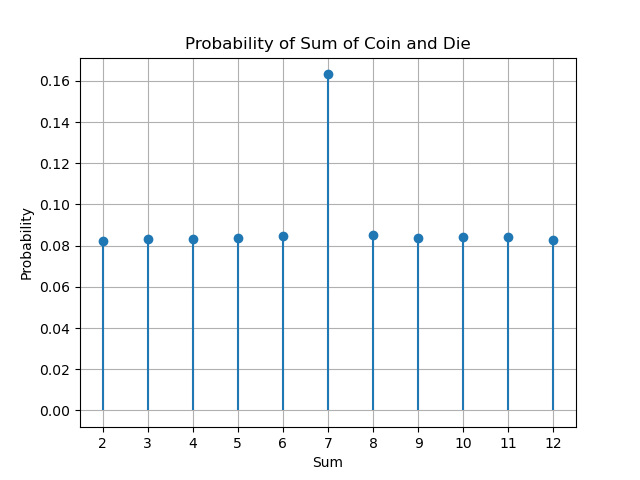
\includegraphics[width=\columnwidth]{figs/Figure_1.png}
		\caption{Solution of the system of linear equations}
		\label{stemplot}
	\end{figure}
\end{document}
